% Preamble --------------------------------------------------------------
\documentclass[aspectratio=169,10pt]{beamer}

% Template --------------------------------------------------------------
% Font ------------------------------------------------------------------

\usepackage[sfdefault, light]{FiraSans} % Fira Sans for text
\usefonttheme[onlymath]{serif}          % Regular LaTeX font for math

% Utilities -------------------------------------------------------------

\usepackage{etoolbox} % for \ifbool and \patchcmd (portability/safety)

% Basic formatting ------------------------------------------------------

\setbeamertemplate{navigation symbols}{}

\setbeamersize{
  text margin left  = 1em,
  text margin right = 1em
} % Margins

\setbeamercovered{transparent} % Pauses in gray

% Colors ----------------------------------------------------------------
% (Define these in your preamble if not already defined)
% \definecolor{main}{RGB}{34, 87, 164}
% \definecolor{secondary}{RGB}{217, 115, 13}

\setbeamercolor{structure}{fg = main}

% Highlight commands
\newcommand{\main}[1]{\textcolor{main}{#1}}           % main highlight
\newcommand{\secondary}[1]{\textcolor{secondary}{#1}} % secondary highlight

% Links and references --------------------------------------------------

\hypersetup{
  colorlinks = true,
  citecolor  = main,
  linkcolor  = main,
  urlcolor   = main
}

\usepackage{natbib}

\let\oldbibitem\bibitem
\renewcommand{\bibitem}{\setlength{\itemsep}{0.8\baselineskip}\oldbibitem}

% Slide numbering / appendix flags --------------------------------------

\makeatletter

% Flag: are we in the appendix?
\newif\ifinappendix
\inappendixfalse

% Global toggle for slide numbers
\newif\ifshowslidenumbers
\showslidenumberstrue % default: show numbers

% User-level command: \slidenumbering{true} or \slidenumbering{false}
\newcommand{\slidenumbering}[1]{%
  \csname showslidenumbers#1\endcsname
}

% Foot text (left side of footline)
\newcommand\foottext[1]{\gdef\beamer@foottext{#1}}
\gdef\beamer@foottext{}

\setbeamertemplate{footline}{%
  \ifbool{beamer@plainframe}{%
  }{%
    \scriptsize
    \hspace{0.15cm}%
    {\usebeamercolor[fg]{structure}\beamer@foottext}%
    \hfill
    % No slide numbers in appendix; main part uses main-frame total only
    \ifinappendix
      % nothing
    \else
      \ifshowslidenumbers
        {\usebeamercolor[fg]{structure}\insertframenumber/\insertmainframenumber}%
      \fi
    \fi
    \hspace{0.6em}\vspace{0.6em}%
  }%
}

\makeatother

% Title page ------------------------------------------------------------

\setbeamerfont{title}{series    = \bfseries}
\setbeamerfont{subtitle}{series = \bfseries}

\setbeamerfont{subtitle}{size  = \large}
\setbeamerfont{institute}{size = \normalsize}

% Sections --------------------------------------------------------------

\AtBeginSection[]{%
  \begin{frame}[plain, noframenumbering]%
    \centering%
    {\Large\bfseries\usebeamercolor[fg]{structure}\insertsection}%
  \end{frame}%
}

% Lists -----------------------------------------------------------------

\setbeamertemplate{itemize item}{$\bullet$}
\setbeamertemplate{itemize subitem}{$\circ$}
\setbeamertemplate{itemize subsubitem}{--}

\makeatletter

\newcommand{\beamer@setitemsep}{%
  \ifnum\@itemdepth = 1\relax
    \setlength{\itemsep}{1em}%
  \else\ifnum\@itemdepth = 2\relax
    \setlength{\itemsep}{0.35em}%
  \fi\fi
  % depth >= 3: leave beamer defaults
}

\let\beamer@origitemize\itemize
\def\itemize{\@ifnextchar[{\beamer@itemize}{\beamer@itemize[]}}
\def\beamer@itemize[#1]{%
  \beamer@origitemize[#1]%
  \beamer@setitemsep
}

\let\beamer@origenumerate\enumerate
\def\enumerate{\@ifnextchar[{\beamer@enumerate}{\beamer@enumerate[]}}
\def\beamer@enumerate[#1]{%
  \beamer@origenumerate[#1]%
  \beamer@setitemsep
}

\makeatother

% References ------------------------------------------------------------

\newcommand{\bibfile}[1]{\def\thebibfile{#1}}

\makeatletter
\newcommand{\references}{%
  % NO \section or \section* here -> nothing new added to the section navigation bar

  % Manual "section slide" (same style as your \AtBeginSection)
  \begin{frame}[plain, noframenumbering]
    \centering
    {\Large\bfseries\usebeamercolor[fg]{structure}References}
  \end{frame}

  \begingroup
  % Prevent BibTeX/thebibliography from creating its own heading/entry
  \renewcommand{\refname}{}%
  \@ifundefined{bibsection}{}{%
    \renewcommand{\bibsection}{}%
  }%

  \begin{frame}[allowframebreaks, plain, noframenumbering]{References}
    \footnotesize
    \bibliographystyle{ecta}
    \bibliography{\thebibfile}
  \end{frame}%
  \endgroup
}
\makeatother

% Appendix ---------------------------------------------------------------
% Single appendix redefinition (sets flag + creates Appendix section)

\makeatletter
\let\beamer@origappendix\appendix
\renewcommand{\appendix}{%
  \beamer@origappendix%
  \inappendixtrue%
  \section{Appendix}%
}
\makeatother

% Top-right section index (clickable, gray) -----------------------------

% --- TOC bar toggle -----------------------------------------------------
\newif\iftocbar
\tocbartrue % default (can be overridden in main.tex)

\newcommand{\tocbar}[1]{%
  \csname tocbar#1\endcsname % expects 'true' or 'false'
}

% --- TOC bar style ------------------------------------------------------
\setbeamercolor{section in head/foot}{fg=gray}
\setbeamercolor{section in head/foot shaded}{fg=gray}
\setbeamerfont{section in head/foot}{size=\scriptsize}

\newlength{\secnavrightmargin}
\setlength{\secnavrightmargin}{-0.4em} % adjust right margin here

\makeatletter
\setbeamertemplate{headline}{%
  \iftocbar
    \ifbool{beamer@plainframe}{}{%
      \ifinappendix\else
        \vspace*{2em}%
        \begin{beamercolorbox}[wd=\paperwidth, ht=0em, dp=0em]{section in head/foot}%
          \begingroup
          \hypersetup{linkcolor=gray}%
          \hfill%
          \insertsectionnavigationhorizontal{\dimexpr\paperwidth-\secnavrightmargin\relax}{}{}%
          \kern\secnavrightmargin%
          \endgroup
        \end{beamercolorbox}%
        \vspace*{-1em}%
      \fi
    }%
  \fi
}
\patchcmd{\sectionentry}{\hskip1.875ex plus 1fill}{\hskip1em}{}{}
\makeatother

% -----------------------------------------------------------------------


% Extra packages --------------------------------------------------------
\usepackage{booktabs}
\usepackage{array}
\usepackage{tikz}
\usetikzlibrary{arrows.meta,positioning,calc}
\usepackage{tcolorbox}

% Colors ----------------------------------------------------------------
\definecolor{main}{RGB}{34, 87, 164}
\definecolor{secondary}{RGB}{217, 115, 13}
\definecolor{good}{RGB}{91, 138, 114}     % muted green for "implemented"
\definecolor{bad}{RGB}{168, 58, 58}       % muted red for "open"

\bibfile{references}

% Title page ------------------------------------------------------------
\title{Master Thesis Preliminary Results}
\subtitle{Asymmetric-granularity friction in Spanish electricity markets}
\author{Pablo Paramio P\'erez \\ Advisor: Pedro Mira}
\institute{CEMFI}
\date{\today}

% TikZ styles -----------------------------------------------------------
\tikzset{
  mybox/.style={
    draw=main, very thick, rounded corners=2pt,
    fill=main!6, align=center, inner sep=5pt
  },
  mybox2/.style={
    draw=secondary, very thick, rounded corners=2pt,
    fill=secondary!10, align=center, inner sep=5pt
  },
  arr/.style={-Latex, very thick, draw=main},
  arr2/.style={-Latex, very thick, draw=secondary},
  lab/.style={font=\scriptsize}
}

% ======================================================================
\begin{document}

% ----------------------------------------------------------------------
\begin{frame}[plain, noframenumbering]
  \titlepage
\end{frame}

% ======================================================================
\section{Recap and IO question}

% ----------------------------------------------------------------------
\begin{frame}{Recap: Spain's 2024--2025 reform sequence}
\begin{columns}[T]
\column{0.46\textwidth}
\begin{itemize}
  \item Three reform stages staggered the move from MTU60 (hourly) to MTU15 (quarter-hourly):
  \begin{itemize}
    \item \textbf{Dec 2024}: ISP15 (imbalance settlement)
    \item \textbf{Mar 2025}: ID15 (intraday trading)
    \item \textbf{Oct 2025}: DA15 (day-ahead trading)
  \end{itemize}
  \item This created a \textbf{10-month asymmetric-granularity window} (Dec 2024 -- Sep 2025) where settlement was 15-min while DA cleared at 60-min.
  \item Plus the \secondary{April 28 2025 blackout} during DA60/ID15 -- a confound we have to account for.
\end{itemize}

\column{0.54\textwidth}
\centering
\small
\renewcommand{\arraystretch}{1.15}
\begin{tabular}{>{\raggedright\arraybackslash}p{2.05cm} >{\centering\arraybackslash}p{1.05cm} >{\centering\arraybackslash}p{1.05cm} >{\centering\arraybackslash}p{1.05cm}}
\toprule
\textbf{Period} & \textbf{ISP} & \textbf{DA} & \textbf{ID} \\
\midrule
Pre-Dec 2024         & 60 & 60 & 60 \\
Dec24--Mar25 \footnotesize{(ISP15-win)} & 15 & 60 & 60 \\
Mar25--Sep25 \footnotesize{(DA60/ID15)} & 15 & 60 & 15 \\
Oct25 onward \footnotesize{(DA15/ID15)}   & 15 & 15 & 15 \\
\bottomrule
\end{tabular}

\vspace{1.6em}
\centering
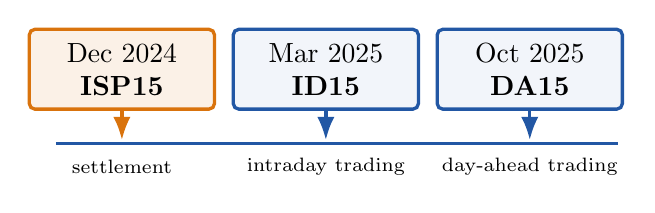
\begin{tikzpicture}[x=0.7cm,y=0.9cm]
\draw[very thick, draw=main] (-5.1,0) -- (5.1,0);

\node[mybox2, text width=2cm] (d24) at (-3.9,1.05) {Dec 2024\\ \textbf{ISP15}};
\draw[arr2] (d24.south) -- (-3.9,0.05);

\node[mybox, text width=2cm] (m25) at (-0.2,1.05) {Mar 2025\\ \textbf{ID15}};
\draw[arr] (m25.south) -- (-0.2,0.05);

\node[mybox, text width=2cm] (o25) at (3.5,1.05) {Oct 2025\\ \textbf{DA15}};
\draw[arr] (o25.south) -- (3.5,0.05);

\node[lab] at (-3.9,-0.33) {settlement};
\node[lab] at (-0.2,-0.33) {intraday trading};
\node[lab] at (3.5,-0.33) {day-ahead trading};
\end{tikzpicture}
\end{columns}
\end{frame}

% ----------------------------------------------------------------------
\begin{frame}{From the February proposal to today's findings}
\begin{itemize}
  \item In February I proposed a \textbf{theoretical extension of \citet{ItoReguant}}, predicting:
  \begin{itemize}
    \item \textbf{DA15} is the key reform that smooths imbalances.
    \item \textbf{Dispersion} risk concentrates in the transitional DA60/ID15 window.
    \item Finer granularity creates winners and losers across heterogeneous portfolios.
  \end{itemize}
  \item Today: all three predictions are \textbf{empirically confirmed} -- but the surviving microfoundation is system-layer settlement-clock mismatch, \textbf{not} the firm-level Allaz--Vila commitment-value channel.
\end{itemize}

\vspace{0.4em}
\begin{tcolorbox}[
  title=Today's IO question,
  colback=main!4, colframe=main, fonttitle=\bfseries
]
When the regulator changes settlement and trading clocks asymmetrically, \textbf{who pays the resulting friction, who captures the rent, and is the rule incentive-compatible} with marginal social cost?
\end{tcolorbox}
\end{frame}


% ======================================================================
\section{Data and empirical strategy}

% ----------------------------------------------------------------------
\begin{frame}{Data and empirical strategy}
\begin{columns}[T]
\column{0.55\textwidth}
\begin{itemize}
  \item \textbf{OMIE bid-level data (Detalle de las ofertas)} -- 6 yrs, 3-month publication lag (current to Jan 2026).
  \item \textbf{ENTSO-E TP}: A85 imbalance prices/volumes; A87 financial balance; A73 per-unit dispatch; A75 wind+solar; A65 D-1 load; A11 cross-border flows.
  \item \textbf{ESIOS (REE)}: \texttt{liquicomun} settlement bundle (181 families, 4.4M rows post-extension); per-BSP aFRR settlement; restrictions/redispatch.
  \item \textbf{Controls}: AEMET weather, CO$_2$/fuels, reservoir filling, installed capacity, French DA prices for the cross-country placebo.
\end{itemize}

\column{0.45\textwidth}
\textbf{Empirical strategy (per Feb deck)}:
\begin{itemize}
  \item No clean external counterfactual -- most European markets adopted MTU15.
  \item \textbf{Same-calendar-month pre-IDA baseline} + bootstrap CIs.
  \item \textbf{Cross-country placebo} (Spain vs France).
  \item Blackout-split robustness (PRE/POST 2025-04-28).
  \item OVB-cleaning under good/bad-control distinction.
\end{itemize}

\vspace{0.4em}
\begin{block}{Status}
\footnotesize
The 3-month OMIE bid-data lag limits firm-level analysis post-Jan 2026; today's system-layer findings use ENTSO-E + ESIOS data current to April 2026.
\end{block}
\end{columns}
\end{frame}


% ======================================================================
\section{Findings: system-layer reform impact}

% ----------------------------------------------------------------------
\begin{frame}{Result 1 -- Four ENTSO-E system metrics jump concordantly at ISP15}
\begin{columns}[T]
\column{0.62\textwidth}
\centering

\includegraphics[width=\linewidth]{../figures/fig01_S5_four_panel_concordance.pdf}

\column{0.38\textwidth}
\begin{itemize}
  \item Monthly system metrics with calendar-month FE, regime contrasts vs same-calendar pre-IDA baseline (78 months).
  \item \textbf{A87} net imbalance settlement income.
  \item \textbf{A86} mean $|V_{\text{imb}}|$.
  \item \textbf{A85} imbalance-price $\sigma$.
  \item \textbf{A84} mean activation price.
\end{itemize}
\vspace{0.3em}
\begin{block}{Joint null}
The four metrics jump concordantly at ISP15 and moderate at MTU15-DA -- this isn't one outlier metric.
\end{block}
\end{columns}
\end{frame}


% ----------------------------------------------------------------------
\begin{frame}{Result 2 -- The headline: \textbf{€1{,}094.9M BRP$\to$TSO settlement transfer}}
\begin{columns}[T]
\column{0.65\textwidth}
\centering

\includegraphics[width=\linewidth]{../figures/fig02_S6_settlement_transfer_headline.pdf}

\column{0.35\textwidth}
\begin{itemize}
  \item \textbf{€1{,}094.9M} cumulative excess (A87 net) over the 10-month asymmetric window vs same-cal pre-IDA baseline.
  \item Bootstrap null CI \textbf{$[-90, +73]$ M€}; observed $\approx 15\times$ upper bound.
  \item Excess collapses to \textbf{€7.4M/mo} (8\% of DA60/ID15 level) at MTU15-DA.
\end{itemize}

\vspace{0.3em}
\begin{block}{Caveat}
\footnotesize
This is a settlement \textbf{redistribution} (BRP$\to$TSO, recycled to consumers via tariff with $\sim$1-yr lag), \textbf{not a deadweight loss}. Welfare interpretation requires a counterfactual on tariff pass-through (out of scope today).
\end{block}
\end{columns}
\end{frame}


% ----------------------------------------------------------------------
\begin{frame}{Result 3 -- Mechanism: forecast-error $\to$ imbalance pass-through}
\begin{columns}[T]
\column{0.62\textwidth}
\centering

\includegraphics[width=\linewidth]{../figures/fig03_B6_passthrough_by_regime.pdf}

\column{0.38\textwidth}
\begin{itemize}
  \item Slope of $|V_{\text{imb}}|$ on $|$wind+solar forecast error$|$, month + hour FE.
  \item \textbf{Pre-IDA-late}: $R^2 = 0.023$ (clean baseline).
  \item \textbf{DA60/ID15 PRE-blackout}: $R^2 = 0.171$ (\textbf{7$\times$} clean reform).
  \item \textbf{DA60/ID15 POST-blackout}: $R^2 = 0.365$ (16$\times$, blackout amplification).
  \item \textbf{DA15/ID15}: $R^2 = 0.028$ -- \textbf{the cleanest reform signature}.
\end{itemize}

\vspace{0.3em}
\begin{block}{Reading}
\footnotesize
Under asymmetric clocks, BRPs cannot match within-hour forecast errors $\to$ they propagate mechanically into imbalance volumes. Symmetric clocks at MTU15-DA close the channel -- even with operación reforzada still in effect.
\end{block}
\end{columns}
\end{frame}


% ----------------------------------------------------------------------
\begin{frame}{Result 4 -- Pigouvian incidence: who actually pays?}
\centering

\includegraphics[width=0.94\linewidth]{../figures/fig06_S7_pigouvian_incidence.pdf}

\vspace{-0.4em}
\begin{itemize}
  \footnotesize
  \item Direct dual-pricing decomposition: per-segment € from signed imbalance $\times$ \texttt{prdvbaqh}/\texttt{prdvsuqh}; reproduces 78\% of system total ($\rho = 0.93$).
  \item \textbf{Pigouvian counterfactual}: charge each segment its $\beta$ marginal contribution to system imbalance cost.
  \item \textbf{LIB free-market retailers + wind} overpay \textbf{$\approx$€141M}; \textbf{conv-RZ + COR + hydro RE} underpay \textbf{$\approx$€159M}.
\end{itemize}
\end{frame}


% ----------------------------------------------------------------------
\begin{frame}{Result 5 -- The structural finding: regime-invariance}
\centering

\includegraphics[width=0.94\linewidth]{../figures/fig07_burden_share_regime_invariance.pdf}

\vspace{-0.5em}
\begin{tcolorbox}[colback=main!4, colframe=main, fonttitle=\bfseries, title=The IO bite]
\footnotesize
\textbf{Wind + LIB free-market retailers consistently pay 60--65\%} of imbalance settlement € in EVERY post-ISP15 regime, including post-MTU15-DA. \textbf{Clock-symmetry shrinks the SCALE of the redistribution but does not relieve its STRUCTURE.}
\end{tcolorbox}
\end{frame}


% ----------------------------------------------------------------------
\begin{frame}{Result 6 -- Cross-country placebo (the Feb proposal said wasn't yet available)}
\begin{columns}[T]
\column{0.62\textwidth}
\centering

\includegraphics[width=\linewidth]{../figures/fig04_B7_france_placebo.pdf}

\column{0.38\textwidth}
\begin{itemize}
  \item Within-day DA price standard deviation by regime, Spain vs France.
  \item \textbf{Spain responds 2--3$\times$ more than France} across reform dates ($\Delta_{ES} = +13.7$ to $+19.7$ €/MWh; $\Delta_{FR} = +5.6$ to $+8.8$).
  \item France didn't undergo MTU15 in our window $\Rightarrow$ Spain-specific shock identified.
\end{itemize}
\vspace{0.3em}
\begin{block}{Caveat}
\footnotesize
The post-2025-04-28 blackout was also Spain-specific. Blackout-split (next slide) addresses this.
\end{block}
\end{columns}
\end{frame}


% ----------------------------------------------------------------------
\begin{frame}{Robustness -- the asymmetric-friction story is reform-driven, not blackout-driven}
\begin{columns}[T]
\column{0.62\textwidth}
\centering

\includegraphics[width=\linewidth]{../figures/fig05_S6_blackout_robustness.pdf}

\column{0.38\textwidth}
\begin{itemize}
  \item \textbf{Clean April 2025} (PRE-blackout, single month): \textbf{+€75.7M} excess.
  \item \textbf{May--Sep 2025} (POST-blackout DA60/ID15): €93.5M/mo (+24\% vs clean April -- modest amplification, not source).
  \item \textbf{Oct--Dec 2025} (DA15/ID15, post-blackout still in effect): \textbf{€7.4M/mo}.
\end{itemize}
\vspace{0.3em}
\begin{block}{Key signature}
\footnotesize
The DA15/ID15 collapse holds \textbf{despite} operación reforzada in effect -- friction is reform-driven, not blackout-driven.
\end{block}
\end{columns}
\end{frame}


% ======================================================================
\section{Synthesis}

% ----------------------------------------------------------------------
\begin{frame}{Two policy levers, two distinct mechanism-design failures}

\begin{tcolorbox}[colback=good!8, colframe=good, fonttitle=\bfseries,
  title={Lever 1 -- Clock-symmetry  \hfill \textcolor{good}{\textbf{IMPLEMENTED}}}]
\footnotesize
\textbf{Failure}: asymmetric clock scales create a BRP$\to$TSO transfer of \textbf{€1.1B} over 10 months. \\
\textbf{Lever}: clock-symmetry at MTU15-DA. \\
\textbf{Effect}: reduces total scale 6$\times$ (€91M/mo $\to$ €7.4M/mo). \\
\textbf{Identification}: same-calendar-month pre-IDA baseline + bootstrap (Result 2); microfoundation from forecast-error $\to$ imbalance volume pass-through R$^2$ collapse (Result 3); cross-country placebo (Result 6); blackout robustness (Result 7).
\end{tcolorbox}

\begin{tcolorbox}[colback=bad!8, colframe=bad, fonttitle=\bfseries,
  title={Lever 2 -- Settlement-rule redesign \hfill \textcolor{bad}{\textbf{OPEN}}}]
\footnotesize
\textbf{Failure}: non-Pigouvian uniform-rate allocation across heterogeneous-MC segments. \\
\textbf{Lever}: settlement-rule redesign (Pigouvian per-segment pricing). \\
\textbf{Status}: not addressed by clock-symmetry. Wind + LIB retailers pay 60--65\% of imbalance € in \emph{every} post-ISP15 regime, including post-MTU15-DA (Result 5). \\
\textbf{Implementation challenges}: real-time per-segment marginal-cost measurement; trade-off with BRP forecast-accuracy incentives. Open mechanism-design problem, not a clean policy intervention.
\end{tcolorbox}
\end{frame}


% ----------------------------------------------------------------------
\begin{frame}{What this talk does \emph{not} show}
\begin{itemize}
  \item Today's findings are the \textbf{system-layer reform-impact slice}. The thesis maps three additional IO channels covered in Parts II--IV:
  \begin{itemize}
    \item \textbf{Firm-level structural market power} -- IB DA cleared-price-difference rent $\sim$€820M post-MTU15-IDA, regime-invariant. Hydro Cournot-pivotality at 63\% of post-MTU15-IDA hours \citep{Bushnell2003,HortacsuPuller2008,CiarretaEspinosa2010}.
    \item \textbf{Cross-market firm specialisation} -- IB$\to$DA hydro Cournot; \textbf{GE$\to$aFRR} (€13.8M revenue post-MTU15-DA, +52\% above IB); \textbf{Naturgy$\to$CCGT generation} post-blackout (+7.1pp share gain).
    \item \textbf{Post-CNMC strategic-availability conduct} -- 13-yr CNMC enforcement record; replication of the 2023 SBO3 three-situation pivotality test shows Naturgy fleet-wide bid-price wedge of 11--35\% in zone-pivotal hours; SBO3 itself still +14\% post-sanction \citep{JoskowKahn2002}.
  \end{itemize}
  \item These findings \textbf{pre-date and survive} the MTU15 reform -- they don't fit the reform-impact frame of this talk.
\end{itemize}
\end{frame}


% ======================================================================
\section{Conclusions and next steps}

% ----------------------------------------------------------------------
\begin{frame}{Conclusions}
\begin{enumerate}
  \item Spain's MTU15 reform sequence is \textbf{empirically tractable} via same-cal pre-IDA baseline + cross-country placebo; the Feb-deck \citet{ItoReguant} predictions hold at \textbf{€1.1B order of magnitude}.

  \item The reform reveals \textbf{two distinct mechanism-design failures}:
  \begin{itemize}
    \item \textbf{Lever 1 (clock-symmetry)}: implemented at MTU15-DA, reduces scale 6$\times$.
    \item \textbf{Lever 2 (settlement-rule redesign)}: open, structural correlation between renewable forecast errors and system imbalance direction (\textbf{LIB retailer correlation 0.74--0.81}) means renewables systematically face the penalty side of dual pricing.
  \end{itemize}

  \item The asymmetric-granularity friction \textbf{is reform-driven, not blackout-driven}: clean PRE-blackout April 2025 alone is +€75.7M; post-MTU15-DA collapse holds despite operación reforzada.
\end{enumerate}
\end{frame}


% ----------------------------------------------------------------------
\begin{frame}{Next steps}
\begin{itemize}
  \item \textbf{Structural model extension}: distinguish \emph{scale} (clock-symmetry) from \emph{structure} (Pigouvian incidence) levers; quantify implementation trade-offs of segment-conditional pricing.
  \item \textbf{Brodersen-style Bayesian structural time series counterfactual} \citep{Brodersen_2015,CausalImpact15min} as a complementary identification strategy for the next draft.
  \item \textbf{Per-BRP imbalance settlement verification} -- ESIOS server has been returning HTTP 500 for 2 weeks on the per-BRP cost archive; will retry. Reduced-form per-segment evidence (today's Results 4--5) is interpretable as upper-bound on cross-segment redistribution.
  \item \textbf{Thesis chapters Parts II--IV} -- firm-level structural market power, cross-market specialisation, post-CNMC strategic-availability conduct (separate from today's reform-impact frame).
  \item \textbf{Master thesis structure proposal} drafted; 5-part synthesis of 37 alive findings.
\end{itemize}

\vspace{0.5em}
\begin{block}{Pipeline status}
\footnotesize
Data pipeline current to April 2026: 4.4M-row \texttt{liquicomun\_all} (ESIOS, 181 families); 5M individual mFRR bid records (ENTSO-E, just unlocked via TP File Library); cross-country French imbalance prices integrated.
\end{block}
\end{frame}


% ----------------------------------------------------------------------
\begin{frame}[plain]
  \centering
  \Large Thank you!
  \vspace{1em}

  \normalsize
  Questions and discussion welcome.
\end{frame}


% ======================================================================
\references

\end{document}
